\newpage
\section{Documentation for programmers}
\subsection{Specification}
The program implements a DHCP relay. Figure~\ref{fig:dhcp} depicts how it works.
\begin{figure}[h]
	\centering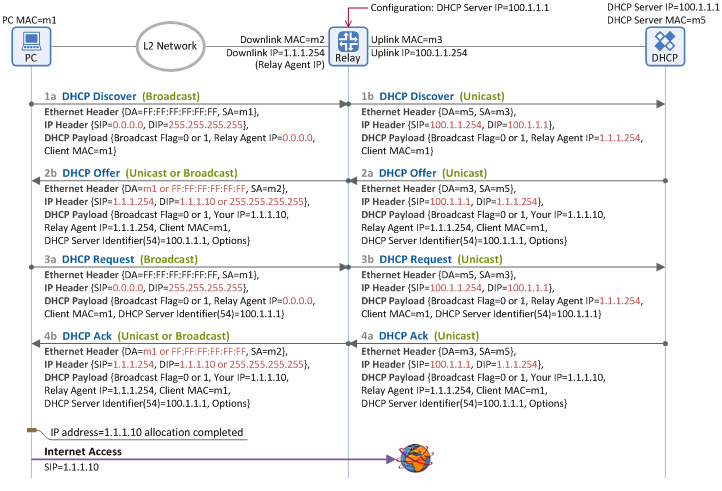
\includegraphics[width=\textwidth]{images/dhcp}
	\caption{Example of DHCP protocol communication\protect\footnotemark}
	\label{fig:dhcp}
\end{figure}
\footnotetext{\url{https://www.netmanias.com/en/?m=view\&id=techdocs\&no=6000}}

Basically, a DHCP relay is a ``man in the middle'' between the client and the DHCP server. It helps the client to contact the server in order to obtain an IP address. It does so receiving the broadcast packets sent by clients and forwarding them in an unicast connection to one (or more) DHCP servers, and vice versa, forwarding the server responses in broadcast to the clients.

A relay slightly modify each packet. The actual changed fields depend on where the packet is coming from, as follows:
\begin{itemize}
	\item \textbf{Server $\rightarrow$ Client}:
	\begin{itemize}
		\item \textbf{Ethernet Payload}
		\begin{itemize}
			\item Destination MAC Address: DHCP Relay Uplink MAC $\to$ Broadcast
			\item Source MAC Address: DHCP Server MAC $\to$ DHCP Relay MAC Address
		\end{itemize} 
		\item \textbf{IP Payload}
		\begin{itemize}
			\item Source IP Address: DHCP Server IP Address $\to$ DHCP Relay Downlink IP
			\item Destination IP Address: DHCP Relay Downlink IP $\to$ Broadcast
		\end{itemize}	
	\end{itemize}
	\item \textbf{Client $\rightarrow$ Server}:
	\begin{itemize}
		\item \textbf{Ethernet Payload}
		\begin{itemize}
			\item Destination MAC Address: Broadcast $\to$ DHCP Server MAC
			\item Source MAC Address: PC MAC Address $\to$ DHCP Relay Uplink MAC 
		\end{itemize}
		\item \textbf{IP Payload}
		\begin{itemize}
			\item Source IP Address: 0.0.0.0 (no IP address) $\to$ DHCP Relay Uplink IP
			\item Destination IP Address: Broadcast $\to$ DHCP Server IP
		\end{itemize}
		\item \textbf{DHCP Payload}
		\begin{itemize}
			\item Gateway IP Address (GIADDR): 0.0.0.0 $\to$ DHCP Relay Downlink IP
		\end{itemize}
	\end{itemize}
\end{itemize}

\subsection{Design}
Our ASG (\textbf{A}synchronous \textbf{S}tate \textbf{G}raphs) diagram is depicted in Figure~\ref{fig:asg}.

\begin{figure}[h]
	\centerline{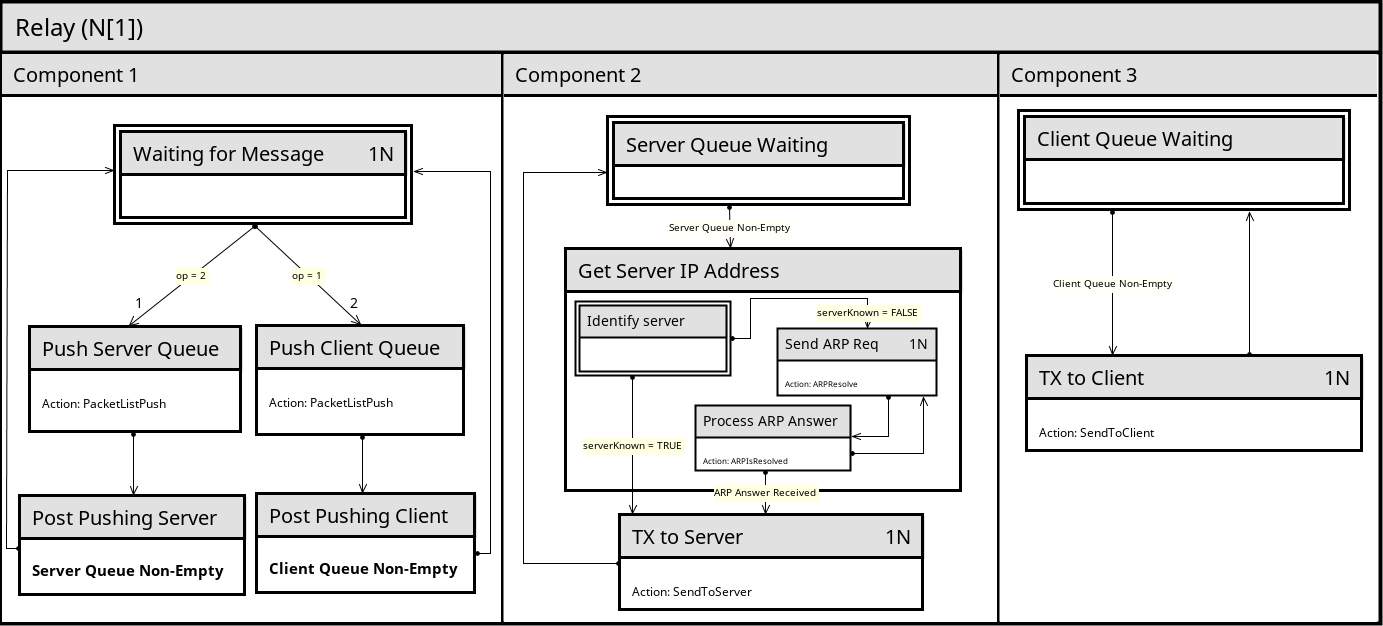
\includegraphics[width=1.15\textwidth]{images/asg-diagram}}
	\caption{ASG diagram modeling a DHCP relay}
	\label{fig:asg}
\end{figure}

The DHCP relay consists of three parallel components following a producer-consumer pattern. Component 1 waits for a packet, either from a client (broadcast) or a server (unicast). Components 2 and 3 then push the modified (note the modification is intended to be a consumer's responsibility, but this is not mandatory) packet in a queue (two different queues are used, respectively for the server and clients). The corresponding consumer polls on its queue in order to detect a new packet. The polling has not to be confused with active waiting, since components are supposed to be parallel: if the queue is empty the corresponding producer simply releases the processor, allowing other components to be dispatched.

Component1's \texttt{WAITING FOR PACKETS} state has got two outgoing transitions. If both of them may be crossed, the ``server'' one goes first. This means in our design the server has a higher priority than the clients. We consider the former to be more important than the latter, since it plays a significant role in the DHCP handshake. The protocol cannot proceed unless at least one server offers an IP address, and clients may retransmit their requests if no answer is received. We assign 2 as a priority to the server transition and 1 to the client one.

Component 2 and 3 are similar in their behavior. The only difference is the ARP request made by Component2 in order to get to know the server MAC address. This is necessary only the first time a client requires an IP address. Afterwards, a boolean flag, \texttt{serverKnown} in the diagram, becomes \texttt{TRUE}, meaning that no ARP requests are needed anymore. Even if this approach only works with one server, it can easily be further extended to work with as many servers as needed, just by using a list or an array.

A different approach might be issuing the ARP request(s) at initialization time. In this way, transmitting a packet to the server would not require an ``on the fly'' request. This is a reasonable solution as soon as the DHCP server(s) is(/are) static. It is our belief that DHCP servers might change dynamically during the lifetime of the relay. Issuing ARP request during the initialization would require a new initialization if a DHCP server is dynamically added. Our solution, on the other hand, does not require any changes or restarts. Supposing to have a procedure to add a server, it would be enough for that procedure to set to \texttt{FALSE} the corresponding \texttt{serverKnown} flag for that server. A correct ARP request will be therefore issued for that server only.

One last point worthy to be explained is the resource \texttt{N} (going for \textit{Network}). The board may only transmit in a half-duplex manner, and it is therefore necessary to allow only one substate at a time to use the network. This is the meaning of \texttt{N}. Each substate accessing the network must acquire \texttt{N} before being allowed to receive or transmit. Every time this happens, \texttt{N} is set to \texttt{TRUE} and the other substates cannot acquire it (thus it is a mutual exclusive resource). If a component $C_1$ needs the network, but the latter is being used by another component $C_2$, $C_1$ has to wait until $C_2$ sets \texttt{N} to \texttt{FALSE} again. There is no risk of deadlock, because there cannot be a circular wait (we only use one resource). In a ``usual'' priority-based scheduling there could be the risk of starvation, meaning that $C_1$ never has the possibility to use the network because a higher priority component acquires it beforehand. Nonetheless, in our design and with our scheduler this cannot happen. For an informal proof of such a claim see \ref{sec:starvation}. 

\newpage
\subsection{LCD non-blocking module}
The key concept in multitasking real-time systems is that tasks must be ``small enough'', in order not to prevent the processor for executing other operations.
In this project it is required to use the LCD display to print information messages, but the C functions provided by Microchip are not optimized for multitasking and take a non negligible time to be processed; the \texttt{LCDBlocking} module has been thus converted in \texttt{LCDNonBlocking} and integrated into the TCP/IP stack to provide a better display handling in an environment with different tasks.\\

The most time-demanding functions in the LCD library (\texttt{LCDInit}, \texttt{LCDErase}, \texttt{LCDUpdate}) have been \textbf{split in smaller states}. When called, the LCD task can only execute a part of a function: the following ones are executed at successive task calls; furthermore, each state can be accessed only if a sufficient amount of time has passed from the previous one, in line with what happened in the original file where some delays were placed between instructions.\\

\begin{wrapfigure}{l}{3.5cm}
	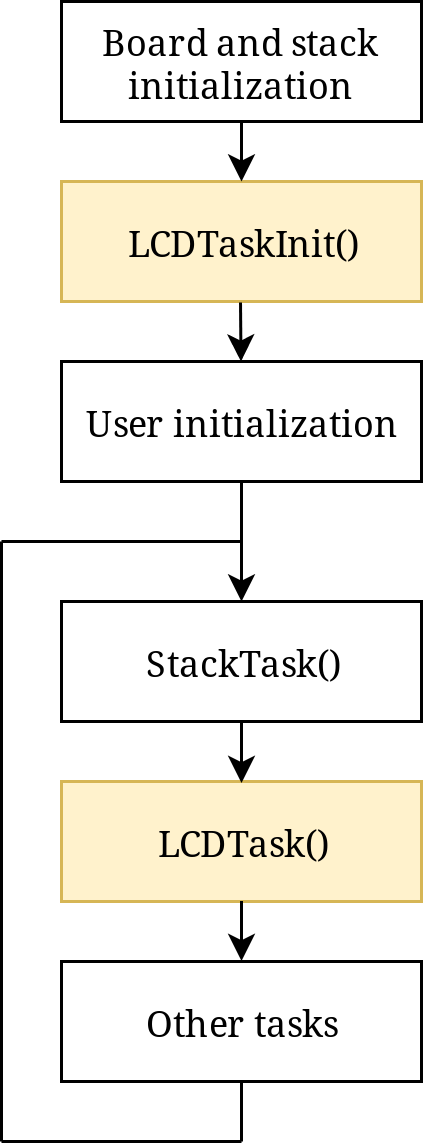
\includegraphics[width=3cm]{images/taskmgmt}
	\label{fig:taskmgmt}
\end{wrapfigure}

The main functions of the new library are \texttt{LCDTaskInit} and \texttt{LCDTask}. The first one is an initialization function which is used to assign default values to control variables and configure the resources needed for the correct operation handling. The latter is the proper task, which runs inside the cooperative multitasking loop.\\
These functions are called in the main entity as a design choice, but they could have also been integrated into the \texttt{StackTsk} file of the TCP/IP stack.\\

The big difference between the new library and the old one is that the operations are not executed immediately but are ``appended'' somewhere, so that the task can pick and perform them in successive steps without losing information about other operation requests happening in the meanwhile.\\
In order to do this, a \textbf{circular list} (actually, a circular array of structures) has been implemented: each time an \textit{Init}, \textit{Erase} or \textit{Update} operation is required, the list is filled with a code representing that operation and the text to write, if needed; this guarantees that the display always reflects the correct history of operations regardless of the state of the shadow copy.\\
The circular list static allocation required the availability of more than 256 bytes in memory, that is the maximum dimension allowed by default due to internal division of databanks in the PIC18. To overcome this limitation, the linker script was modified to create a single databank of twice the size and a \texttt{\#pragma} directive was introduced to memorize the list in that exact memory location; the solution was fully tested and does not introduce any kind of issue.\\


The delay handling is entrusted to \textbf{Timer 1} (external 32.768 kHz oscillator) because it is not used by any other part of the system; the timer is in a bounded configuration and the initial value of the register is calculated according to the necessary minimum delay for each stage. If such a waiting condition is active, the LDC task checks for an overflow of the timer register before proceeding to the execution.\\

The instruction flow of the LCD task is represented in the next page; it is a simple diagram which is not meant to explain the detailed content of each block but the general behavior of the module. For in-depth analysis it is possible to read the code.

\begin{figure}
	\centering
	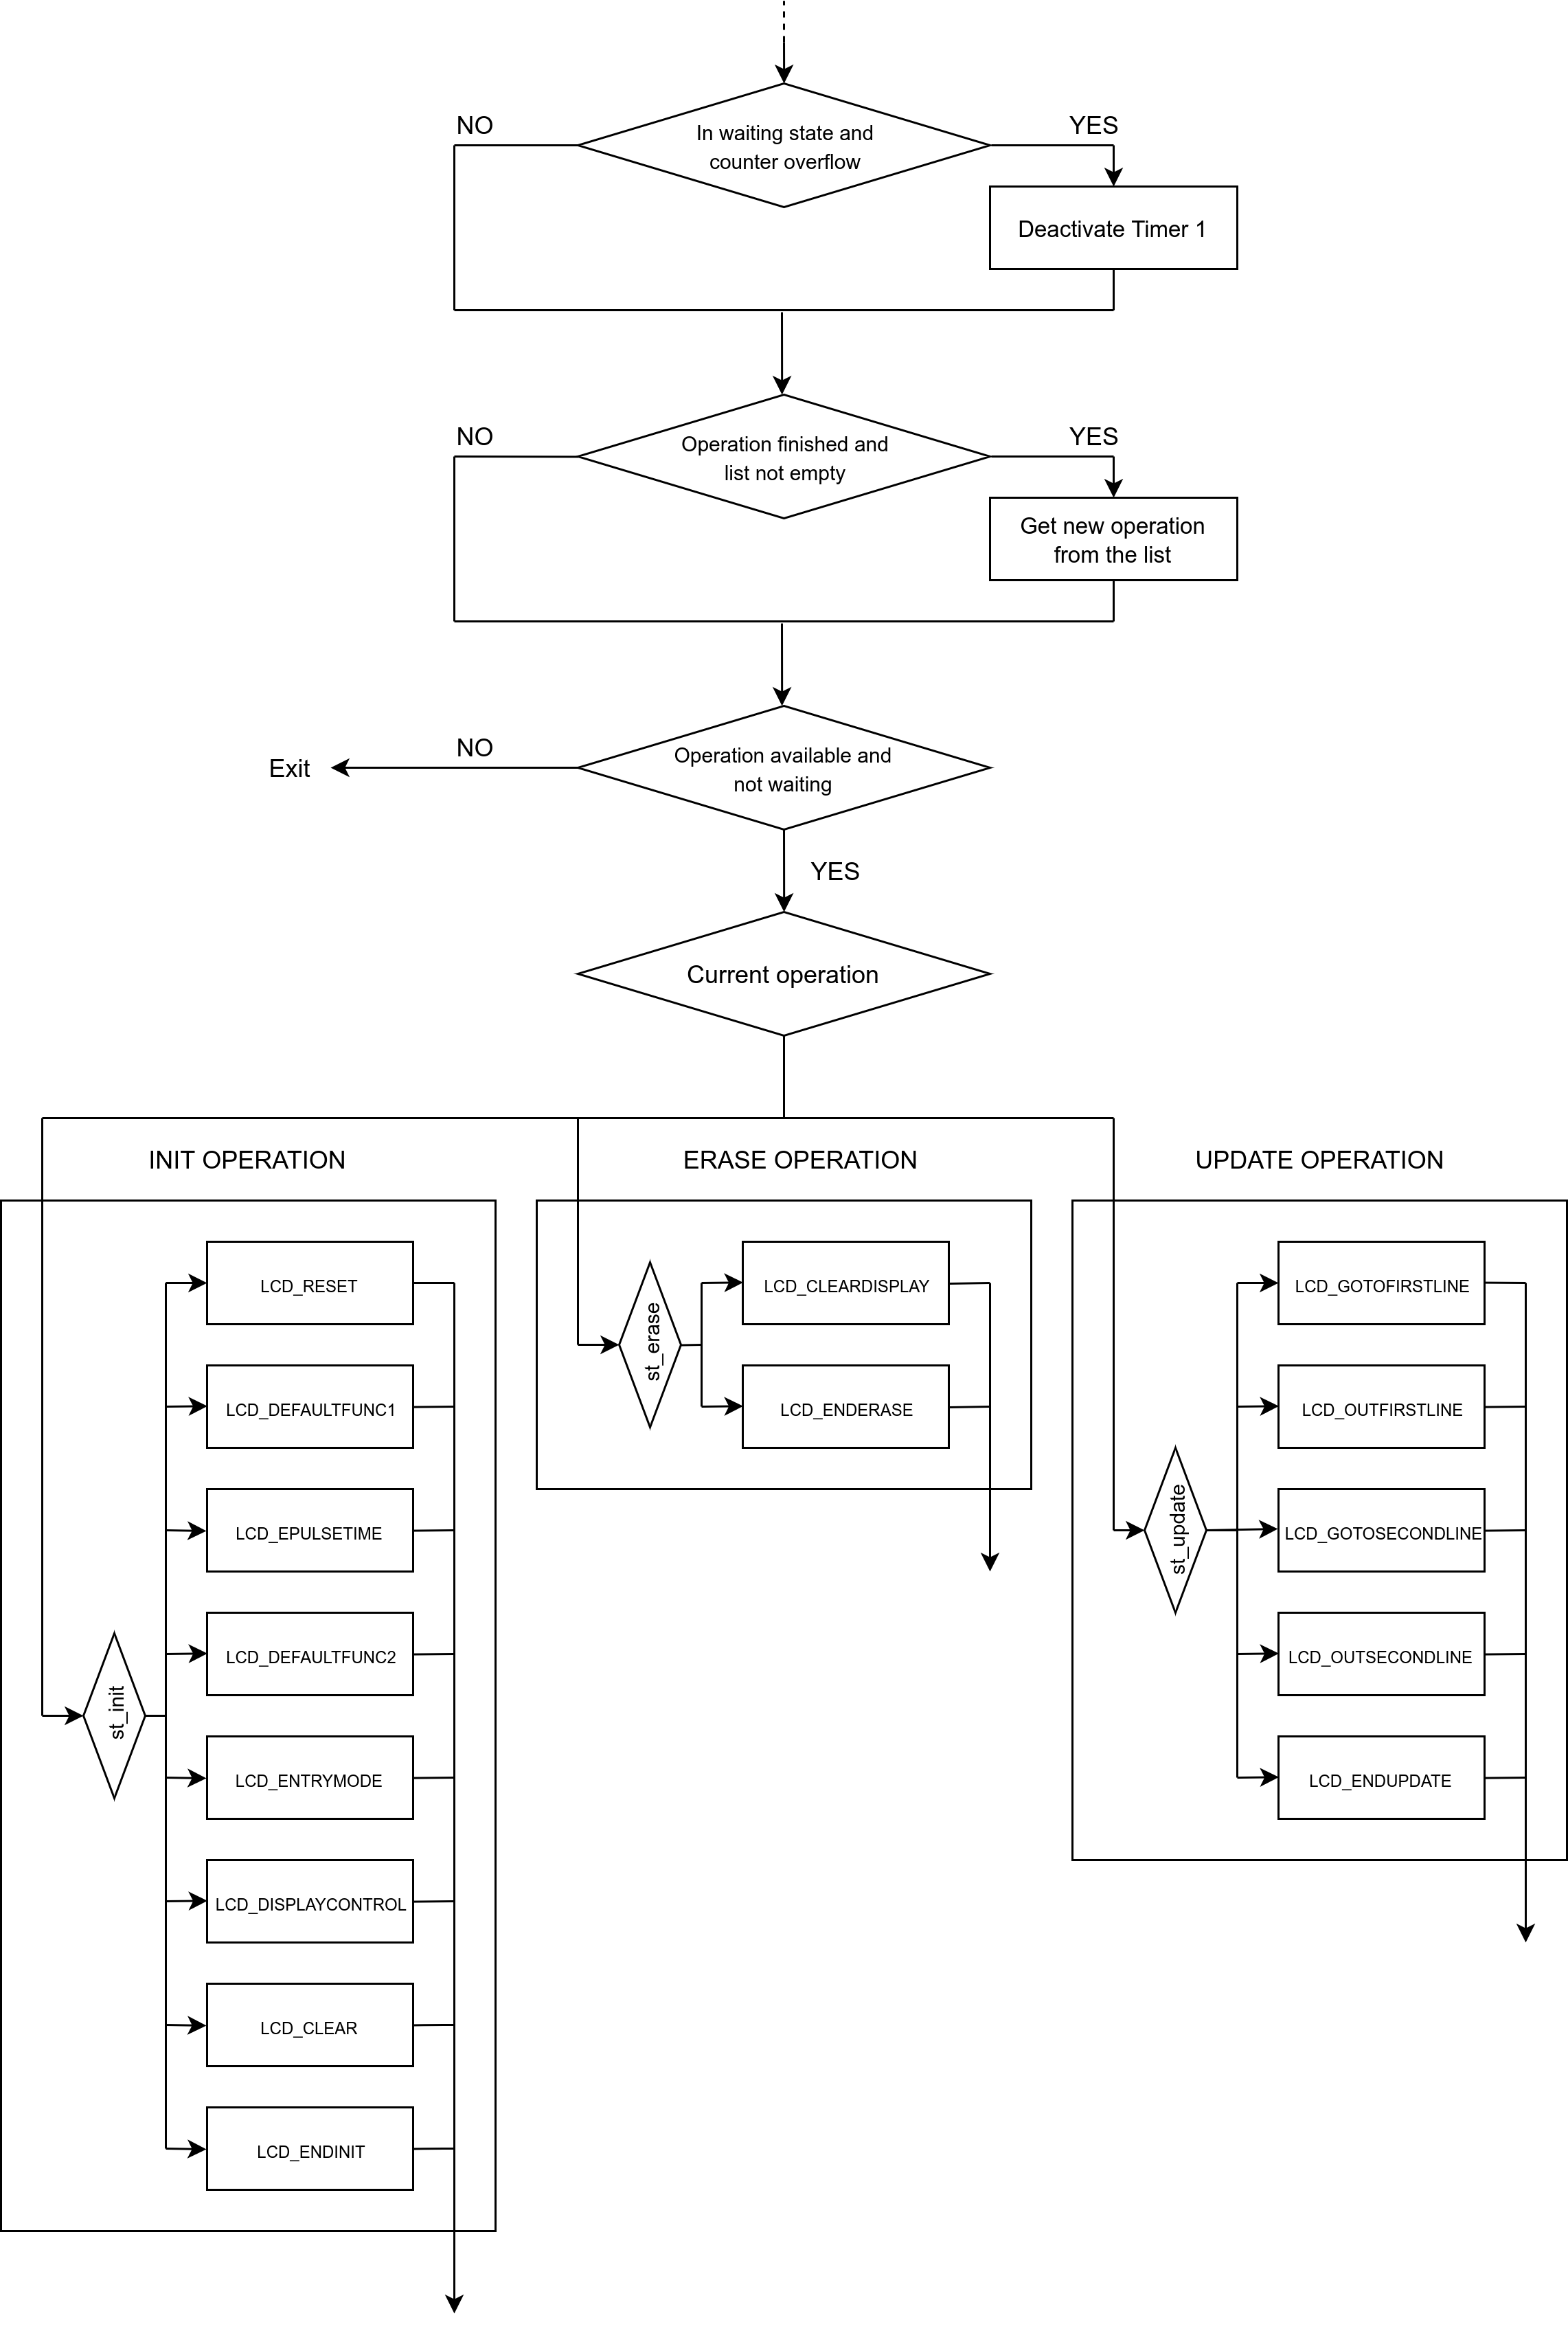
\includegraphics[width=\linewidth]{images/lcdnonblocking2}
	\caption{LCD task instruction flow chart}
	\label{fig:lcdnonblocking2}
\end{figure}

\newpage
\subsection{Relay}
The main entry point for the relay is the file \texttt{DHCPRelay.c}, containing the implementation. Function signatures and \texttt{enum} definitions are in its header file, \texttt{DHCPRelay.h}. The definitions here contained implement the cooperative scheduling. \texttt{Relay} is refined in three main parallel components, representing, respectively, the wait for a message (both form clients and server) and the transmissions. Each \texttt{enum} type corresponds to a component in the ASG diagram. Thus, \texttt{Component1()}, \texttt{Component2()}, and \texttt{Component3()} define the proper actions to be taken when the corresponding component is dispatched. It is not the aim of this document to explain how an ASG diagram should be translated into code, but, in brief, the three function aforementioned should contain a \texttt{switch} checking for the current state and managing actions and transitions accordingly. The C file contains the actual implementations.

Our implementation makes use of two queue in order to store packets incoming both from the server and clients (\texttt{ClientMessages} and \texttt{ServerMessages}). We implement them using a circular list. Seen the limitations in allocating more that 256 bytes and seen the size of the information we store, we decided to set the queues size to 5 (the maximum allowed is 7). An implementation with queues makes the entire managing slightly more difficult. We not only store the DHCP header, but some information used to compose the forwarded message, too. This additional data is the \texttt{MessageType} (i.e. the content of the \texttt{MessageType} option), and the accepted IP address, if any. A boolean flag (\texttt{IPAddressNotNull}) is used to make the distinction. If TRUE, the field \texttt{RequiredAddress} is meaningful. Otherwise, its content is just random bytes.

With fixed-sized queues we may get in trouble when the two ratios (sending are receiving) are not balanced. We decided to manage them with the following policy: if a queue $Q$ is full when a packet is to be pushed (meaning it has already been received) we discard the oldest packet in $Q$. We do not expect this policy to lead to packets loss, since clients usually retransmit their packets if they receive no answer. On the other hand, we do not expect the server queue to be overflowed frequently, since the relay interfaces with only one server. 

We take advantage of \texttt{PacketCircularList}'s \texttt{PacketListIsEmpty} method to simplify the translation from ASG to C. We remove \texttt{POST PUSHING SERVER} and \texttt{POST PUSHING CLIENT} in favor of a direct check on the queue size. This simplifies our program's structure and reduces the overhead (even if small) caused by the ``canonical'' translation of those two states. Hence, the rendez-vous \texttt{Server Queue Non-Empty} and \texttt{Client Queue Non-Empty} are to be translated, respectively, with \texttt{PacketListIsEmpty(\&ServerMessages)} and \\\texttt{PacketListIsEmpty(\&ClientMessages)}.

Please note that the Mikrotik TCP IP stack allows us to ``directly'' modify only the DHCP header. The other modifications the relay should do occur at transmission time.

\subsubsection{Waiting component}
The waiting component is basically a polling on the two open sockets (in the basic implementation we assume there is only one server and client). If enough bytes are written (and ready to be read) in the socket we start the reading procedure, actually implemented by \texttt{GetPacket()}. This function takes two parameters: a pointer to the variable to store the read packet in and the socket to read from. It basically checks if something is waiting in the socket buffer, and, if so, reads the packet (performing a basic check on the hardware type and length). It then reads the options, taking into account only the \texttt{MessageType} and the \texttt{RequestedIPAddress}. If everything works, it returns 0. Otherwise, an error code is given, as follows:
\begin{itemize}
	\item -1 if no packet is available on the selected socket, meaning
there are less then 241 bytes in its buffer;
	\item -2, wrong hardware type          
 	\item -3, wrong hardware length
	\item -4, parameters are invalid
\end{itemize}
The waiting state checks the client and the server socket. It might happen that both of them contain packets ready to be read. In such a scenario, the server as a higher priority and is served first. A flag, \texttt{prevFromClient}, is set to \texttt{TRUE} and checked when the component comes again in the waiting state. If it is \texttt{TRUE}, a client is served; otherwise, both the sockets are checked again. This rules client starvation out.

The final step is pushing the packet into the corresponding queue.

\subsubsection{Transmission to the server}
Transmitting a packet to the DHCP server has two prerequisites: the queue must be not empty and the server MAC address should be known. The former condition becomes \texttt{TRUE} if and only if a packet has not only been received, but pushed into the queue, too. Once a packet is ready, if the server MAC address is not known (meaning \texttt{serverKnown == FALSE}) an ARP request is issued to get to know the address. When a response is received, \texttt{serverKnown} becomes \texttt{TRUE} and no more ARP requests will be issued. Afterwards, the packet is sent to the server via the function \texttt{SendToServer()}. 

\texttt{SendToServer} first checks if the server socket contains enough free space. Socket's remote IP address is set to the server one, and so is the MAC. It pops a packet from its queue and modifies only the \texttt{GIADDR} field, using its own IP address. It sets to 0 every unused field and the magic cookie to the value reported in RFC 1533. The other fields are either taken from the popped packet or generated on the fly. An example of the former is every data contained in the DHCP header, as well as the accepted client IP address, if any. An example of the latter is the subnet mask. The minimum size of such a packet is 300 bytes, in order to ensure compatibility with old DHCP relays that discard
packets smaller than 300 octets. 

\subsubsection{Transmission to the client}
Transmitting a packet to a client is simpler than transmitting to a server. It is indeed not necessary to know any MAC addresses because the packet is sent in broadcast to the client network. Thus, the only prerequisite for this action is a non empty queue. When this is the case, \texttt{SendToClient()} is invoked.

This function operates more or less as \texttt{SendToServer} does, with a few slight differences. The first is the socket remote IP address, which is here set to broadcast (remember the client has not got an IP address unless the very end of the DHCP ``handshake''). The MAC address is correctly set to be the one of the client. The latter value is taken from \texttt{CHADDR}. The second is the magic cookie, set to \texttt{0x63538263}.

\subsubsection{Starvation}\label{sec:starvation}
Suppose Component1 has acquired the network in order to receive a packet, and suppose Component 2 and 3 are waiting for the network in their ``idle'' state. In such a scenario, their queues are not empty. Component1 receives the packet, since it is allowed to use both the network and the processor. In this sense, the receiving operation may be considered as atomic: no one can do anything else since \texttt{GetPacket} never releases the processor and the scheduler is a non-preemptive one. It then executes to completion, and releases both the network (meaning it sets \texttt{N} to \texttt{FALSE}) and the processor. At this point, Component2 has the possibility to acquire the network, and it does so. This means neither Component1 nor Component3 may go ahead with their network-based operations (note that Component1 is now one of its ``push'' substates, which do not require the network). Component2 also does not release neither the network nor the processor during the transmission. It afterwards releases both of them, and Component3 has its chance to proceed. 

If either Component2 or Component3 is not ready to transmit (its queue is empty), it does not compete for \texttt{N}.

This reasoning also applies considering Component2 or Component3 as a starting point. The scheduler always schedule these components in a ``circular'' manner, and there is no chance that a component never executes.

\subsubsection{Enabling the relay mode}
In order to enable the DHCP Relay mode, one should configure the router as said and do small modifications to the definitions provided in the Mikrotik TCP IP stack. In particular, \texttt{STACK\_USE\_DHCP\_CLIENT} and \texttt{STACK\_USE\_DHCP\_SERVER} should be disabled, while \\\texttt{STACK\_USE\_DHCP\_RELAY} should be enabled. These definitions can be found in \texttt{TCPIP.h}.
